
%==========================================================================================
\section{Ressourcenbeschränkte Projektplanung und Zusatzkapazitäten}

\begin{frame}
\frametitle{Gliederung}
\tableofcontents[current] %, hidesubsections]
\end{frame}

\begin{frame}[t]
\frametitle{Ressourcenbeschränkte Projektplanung}
\begin{center}
\includegraphics<1>[page=1, width=\textwidth]{images/rcpsp.pdf}
\includegraphics<2>[page=2, width=\textwidth]{images/rcpsp.pdf}
\includegraphics<3>[page=3, width=\textwidth]{images/rcpsp.pdf}\\
\end{center}

{\small
Projektdauerminimale Einplanung von Arbeitsgängen $j$ mit gegebenen
\begin{itemize}
\itemsep0em
\item<2-3> Dauern $d_j$ \textcolor{gray}{$=(0, 3, 2, 2, 3, 1, 2, 0)$}
\item<3> Ressourcenbelastungen $k_{jr}$ \textcolor{gray}{$=(0, 3, 2, 2, 1, 2, 1, 0)^T$}
\item<2-3> Reihenfolgebeziehungen $i \in \mathcal{P}_j $ \textcolor{gray}{$=(\emptyset, \{0\}, \{0\}, \ldots, \{4,5\}, \{6\})$}
\item<3> Kapazitätsrestriktionen $K_r$ \textcolor{gray}{$=(4)$}
\end{itemize}
}
\end{frame}

%==========================================================================================

\begin{frame}
\frametitle{Projektdauer und Deckungsbeitrag}
\begin{small}
Praxisbeispiel: Aufarbeitung eines Triebwerks durch Dienstleister
\begin{itemize}
\item<1-3> Projektdauer {\large $\downarrow$} $\implies$ Zahlungsbereitschaft {\large $\uparrow$\\}
\item<2-3> Überstunden {\large $\uparrow$} $\implies$ Projektdauer {\large $\downarrow$} Kosten {\large $\uparrow$}\\
\item<3>[] \begin{tabbing}
$\Rightarrow$ \= Maximierung des Deckungsbeitrags als Trade-off zwischen\\
\>Dauer- und Kostenminimierung
\end{tabbing}

\end{itemize}
\end{small}
\begin{center}
\includegraphics<1>[scale=0.29]{images/Erloes.pdf}
\includegraphics<2>[scale=0.29]{images/ErloesKosten.pdf}
\includegraphics<3>[scale=0.29]{images/ErloesKostenDeckungsbeitrag.pdf}
\end{center}
\end{frame}

%%%%%%%%%%%%%%%%%%%%%%%%%%%%%%%%%%%%%%%%%%%%%%%%%%%%%%%%%%%%%%%%%%%%%%%%%%

\begin{frame}
\frametitle{Konzeptionelles Modell: RCPSP\only<2>{-OC}}
\begin{small}
\begin{itemize}
\item Zielfunktion \only<1>{\[\mbox{min } FT_J \textcolor{white}{- \sum_{r \in \mathcal{R}} \sum_{t \in \mathcal{T}} \kappa_r z_{rt}} \]\\[4.5mm]}\only<2>{\textcolor{red}{\[\mbox{max } u_{FT_J} - \sum_{r \in \mathcal{R}} \sum_{t \in \mathcal{T}} \kappa_r z_{rt}\]}}
\item Reihenfolgerestriktionen \[FT_i + d_i \leq FT_j \quad\quad\quad\quad j \in \mathcal{J}, i \in \mathcal{P}_j\]
\item Kapazitätsrestriktionen \[\sum_{j \in \mathcal{S}_t} k_{jr} \leq K_r\only<1>{\textcolor{white}{+ z_{rt}}}\only<2>{\textcolor{red}{+ z_{rt}}} \quad\quad\quad\; r \in \mathcal{R}, t \in \mathcal{T} \]
\[\mathcal{S}_t = \{j\;|\;(FT_j-d_j) < t \leq FT_j\}\]
\item<2> Obere Schranke für Zusatzkapazität \textcolor{red}{\[z_{rt} \leq \overline{z}_r \quad\quad\quad\quad\quad\quad\quad\quad r \in \mathcal{R}, t \in \mathcal{T}\]}
\end{itemize}
\end{small}
\end{frame}

\begin{frame}
\frametitle{Entscheidungsmodell: RCPSP\only<2>{-OC}}
\begin{footnotesize}
\begin{itemize}
\item Zielfunktion\\[-7mm]
\[
		\only<1>{\mbox{min } \sum_{t=EFT_{J+1}}^{LFT_{J+1}} t \cdot x_{{J+1},t} \textcolor{white}{\enspace - \sum_{r \in \mathcal{R}} \sum_{t \in \mathcal{T}} \kappa_r \cdot z_{rt}}}\only<2>{\textcolor{red}{\mbox{max } \sum_{t=EFT_{J+1}}^{LFT_{J+1}} u_t \cdot x_{{J+1},t} - \sum_{r \in \mathcal{R}} \sum_{t \in \mathcal{T}} \kappa_r \cdot z_{rt}}}
\]

\item Einmalige Durchführung
\[
\sum_{t=EFT_j}^{LFT_j} x_{jt} = 1 \,\,\,\quad\quad\quad\quad\quad\quad\quad\quad\quad\quad\quad j \in \mathcal{J}\textcolor{white}{, t \in \mathcal{T}}
\]

\item Reihenfolgerestriktionen
\[
\sum_{t=EFT_i}^{LFT_i} x_{it} \cdot t \leq \sum_{t=EFT_j}^{LFT_j} x_{jt} \cdot t - d_j \,\,\:\:\:\quad\quad\quad j \in \mathcal{J}, \; i \in \mathcal{P}_j
\]

\item Kapazitätsrestriktionen
\[
\sum_{j=1}^{J} \sum_{\tau=t}^{t+d_j-1} k_{jr} \cdot x_{j\tau} \leq K_r\only<1>{\textcolor{white}{ + z_{rt}}}\only<2>{ \textcolor{red}{+ z_{rt}}} \,\,\:\:\:\:\:\quad\quad\quad\quad r \in \mathcal{R}, \; t \in \mathcal{T}
\]

\item<2> Obere Schranke für Zusatzkapazität\\[-3mm]
\[
\textcolor{red}{z_{rt} \leq \overline{z}_r} \,\;\;\quad\quad\quad\quad\quad\quad\quad\quad\quad\quad\quad\quad\quad\quad r \in \mathcal{R}, \; t \in \mathcal{T}
\]
\end{itemize}
\end{footnotesize}
\end{frame}

%%%%%%%%%%%%%%%%%%%%%%%%%%%%%%%%%%%%%%%%%%%%%%%%%%%%%%%%%%%%%%%%%%%%%%%%%%%%%%%%%%

\begin{frame}
\frametitle{Ressoucenbeschränkte Projektplanung\\mit Zusatzkapazitäten (RCPSP-OC)}
\includegraphics<1>[page=1, scale=0.58]{images/RCPSPOCDiagram.pdf}
\includegraphics<2>[page=2, scale=0.58]{images/RCPSPOCDiagram.pdf}\\
\begin{center}

\only<1>{
\begin{tabbing}
Überstundenkosten: \= 0 GE\\
Projektdauer: \> 10 Perioden $\rightarrow$ Erlös: 1 GE\\
Deckungsbeitrag: \> 1 GE - 0 GE = 1 GE
\end{tabbing}
}

\only<2>{
\begin{tabbing}
Überstundenkosten: \= 2 GE\\
Projektdauer: \> 8 Perioden $\rightarrow$ Erlös: 7 GE\\
Deckungsbeitrag: \> 7 GE - 2 GE = 5 GE
\end{tabbing}
}

\end{center}
\end{frame}

%%%%%%%%%%%%%%%%%%%%%%%%%%%%%%%%%%%%%%%%%%%%%%%%%%%%%%%%%%%%%%%%%%%%%%%%%%%%%%%%%%%%%%%%%%%

\begin{frame}
\frametitle{Verwandte Probleme aus der Literatur}
\begin{itemize}
\item Variable Kapazitäten
\begin{itemize}
\item Ressourcenprofil als Parameter {\footnotesize \cite{Klein2000}, \cite{Hartmann2012}}
\item Ressourceninvestitionsproblem {\footnotesize \cite{Mohring1984}}
\item Ressourcenabweichungsproblem {\footnotesize \cite{Neumann2003}} 
\item Ressourcenüberladungsproblem {\footnotesize \cite{Neumann2003}}
\end{itemize}
\vspace*{4mm}
\item Variable Ressourcennachfrage
\begin{itemize}
\item Flexible Ressourcenprofile {\footnotesize \cite{Ranjbar2010}}
\item Zeit-Kosten-Tradeoff-Problem {\footnotesize \cite{Demeulemeester1996}}
\end{itemize}
\end{itemize}

\end{frame}

%==========================================================================================

\section{Heuristische Lösungsverfahren}

\begin{frame}
\frametitle{Gliederung}
\tableofcontents[current] %, hidesubsections]
\end{frame}

\begin{frame}
\frametitle{Notwendigkeit heuristischer Lösung}
\begin{itemize}
\item RCPSP ist $\mathcal{NP}$-schweres Problem
\item und RCPSP $\preceq_p$ RCPSP-OC: $\overline{z}_{r}=0, u_t=-t$
\item[] $\implies$ RCPSP-OC ist $\mathcal{NP}$-schweres Problem\\[10mm]
\item Exakte Lösungsverfahren für praxisnahe Problemgrößen nicht handhabbar
\item[] $\rightarrow$ Heuristik
\end{itemize}
\end{frame}

\begin{frame}
\frametitle{Motivation zur Verwendung eines seriellen Schedule Generation Scheme (SSGS)}
\begin{itemize}
\item Dominierende Heuristiken in Untersuchung von RCPSP-Heuristiken durch {\footnotesize \cite{Kolisch2006}}:\\[6mm] Metaheuristiken basierend auf
\begin{itemize}
\item Seriellem Schedule Generation Scheme (SSGS)
\item Aktivitätenlistenrepräsentation, zum Beispiel:
%\item \textbf{Problem:} SSGS nur anwendbar bei gegebenen Kapazitäten
\end{itemize}
\end{itemize}
\[\lambda=(0,1,2,4,3,5,6,7)\]
\end{frame}

\begin{frame}[t]
\frametitle{Beispiel: Ablauf des SSGS}
\begin{center}
\includegraphics<1>[page=1, width=\textwidth]{images/ssgs.pdf}
\includegraphics<2>[page=2, width=\textwidth]{images/ssgs.pdf}
\includegraphics<3>[page=3, width=\textwidth]{images/ssgs.pdf}
\includegraphics<4>[page=4, width=\textwidth]{images/ssgs.pdf}
\includegraphics<5>[page=5, width=\textwidth]{images/ssgs.pdf}
\includegraphics<6>[page=6, width=\textwidth]{images/ssgs.pdf}
\includegraphics<7>[page=6, width=\textwidth]{images/ssgs.pdf}\\
$\lambda=(0,\textbf<1>{1},\textbf<2>{2},\textbf<3>{4},\textbf<4>{3},\textbf<5>{5},\textbf<6>{6},7)$
\only<7>{
\\[7mm]
\begin{tabular}{l}
\textbf{Problem 1:}\\SSGS nur bei gegebenen Kapazitäten anwendbar
\end{tabular}
}
\end{center}
\end{frame}

\begin{frame}
\frametitle{Bestimmung Aktivitätenliste $\lambda$}
\begin{itemize}
\item[] \textbf{Problem 2:}\\Lösungsgüte von Aktivitätenliste $\lambda$ abhängig\\[7mm]
\item Vollständige Enumeration topologischer Sortierungen nicht handhabbar\\
$\rightarrow$ Suchraum mit Metaheuristik erkunden\\[4mm]
\item Erster Kandidat: Genetischer Algorithmus
\begin{itemize}
\item {\footnotesize 3 der Top 5 RCPSP-Heuristiken nach \cite{Kolisch2006}}
\item {\footnotesize Kann Problem 1 und 2 lösen}
\end{itemize}
\end{itemize}
\end{frame}

\begin{frame}
\frametitle{Genetische Algorithmen}
Repräsentationen im Überblick
\begin{itemize}
	\item Vorbestimmung des Ressourcenprofils\\[2mm]
	\begin{small}
	\begin{tabular}{cp{7.5cm}}
	\hline
	Individuum & Planerzeugung\\
	\hline
	\hline
	 $(\lambda|\tilde{z}_{rt})$ & Nutze möglichst viel ZK, u.B.d.R. $z_{rt} \leq \tilde{z}_{rt}$ \\
	 \hline
	 $(\lambda|\tilde{z}_r)$ &  Nutzbare ZK konstant $z_{rt} \leq \tilde{z}_{r}$\\
	 \hline
	\end{tabular}
	\end{small}\\[4mm]

	\item Auswahl Einplanungszeitpunkt zwischen Reihenfolge- und Ressourcenzulässigkeit\\[2mm]
	\begin{small}
	\begin{tabular}{cp{7.5cm}}
	\hline
	Individuum & Planerzeugung\\
	\hline
	\hline
	$(\lambda|\beta)$& Je AG: Keine ZK oder maximal mögliche\\
	\hline	
	$(\lambda|\tau)$& GA wählt Startzeit in Zeitfenster $\tau \in [0,1)$\\
	\hline
	$(\lambda)$ & Vervollständigung jeder Alternative ohne ZK\\
	\hline
	\end{tabular}
	\end{small}
\end{itemize}


\end{frame}

\begin{frame}
\frametitle{Gemeinsamkeiten der GAs (1/2)}
\begin{itemize}
\item Aktivitätenliste $\lambda$ als Bestandteil der Repräsentation
\item Initialpopulation

\begin{itemize}\item Regret-Based Biased Random Sampling\end{itemize}
\item Kreuzung
	\begin{itemize}
	\item Paarbildung:\\Ziehe zufälliges Paar noch nicht gewählter Individuen\\[4mm]
	\item Tochter (Sohn) per One Point Crossover, d.h.:
	\item[] Übernehme bis zufälliger Stelle $q$ von der Mutter (Vater), Rest in Reihenfolge vom Vater (Mutter)
	\end{itemize}
\end{itemize}
\end{frame}

\begin{frame}
\frametitle{Gemeinsamkeiten der GAs (2/2)}
\begin{itemize}
\item Mutation
\begin{itemize}\item Mit Wahrscheinlichkeit $P_{mutate}$ vertausche AG mit Nachbarn, falls zulässig (Swap Neighborhood)\\[3mm]\end{itemize}
\item Selektion
\begin{itemize}\item Sortiere Gesamtpopulation (Eltern \& Kinder) nach absteigender Fitness. Neue Elterngeneration ist ``vordere'' Hälfte (Ranking Method)\\[3mm]\end{itemize}
\item Fitness \begin{itemize}\item DB von durch Individuum per SSGS induziertem Plan\end{itemize}
\end{itemize}
\end{frame}

\begin{frame}
\frametitle{Bestimmte Zusatzkapazität je\\Ressource und Periode erlauben}

\begin{itemize}
\item Aktivitätenliste um $\tilde{z}_{rt} \in \{0, \ldots, \overline{z}_r \}$ erweitern
\item Für Ressourcenzulässigkeit in SGS zur Verfügung stehende Kapazität: Normalkapazität + $\tilde{z}_{rt}$
\item Möglicher Gebrauch von Überstunden über Planungshorizont \textcolor{red}{\emph{flexibel}}
\end{itemize}

\begin{small}
\begin{center}
\begin{tabular}{rl}
\hline 
Individuum & $(\lambda|\tilde{z}_{rt})=(0,1,3,2,4|\begin{pmatrix} 0 & 2 & 2 & \ldots\\ \vdots & \ddots \end{pmatrix})$\parbox[c][40pt][c]{0pt}{}\tabularnewline
\hline 
Initialpopulation & $\tilde{z}_{rt}=\mbox{rand }0\ldots\overline{z}_{r}\;\forall r,t$\tabularnewline
\hline 
Rekombination & One Point Crossover\tabularnewline
\hline 
Mutation & $\tilde{z}_{rt}=\mbox{rand }0\ldots\overline{z}_{r}$ mit $P_{mutate}$\tabularnewline
\hline 
Fitness & DB von Plan erzeugt durch SSGS\tabularnewline
\hline 
\end{tabular}
\end{center}
\end{small}
\end{frame}

\begin{frame}
\frametitle{Beispiel für $(\lambda|z_{rt})$:\\Einplanung von AG 4}
\includegraphics<1>[page=1, scale=0.8]{images/SSGSzrt.pdf}
\includegraphics<2>[page=2, scale=0.8]{images/SSGSzrt.pdf}
\end{frame}

\begin{frame}
\frametitle{Bestimmte Zusatzkapazität je\\Ressource erlauben}

\begin{itemize}
\item Aktivitätenliste um $\tilde{z}_{r} \in \{0, \ldots, \overline{z}_r \}$ erweitern
\item Für Ressourcenzulässigkeit in SGS zur Verfügung stehende Kapazität: Normalkapazität + $\tilde{z}_{r}$
\item Möglicher Gebrauch von Überstunden über Planungshorizont \textcolor{red}{\emph{konstant}}
\end{itemize}

\begin{small}
\begin{center}
\begin{tabular}{rl}
\hline 
Individuum & $(\lambda|\tilde{z}_{r})=(0,1,3,2,4|0,2,2,0,3,2,1,\ldots)$\parbox[c][40pt][c]{0pt}{}\tabularnewline
\hline 
Initialpopulation & $\tilde{z}_{r}=\mbox{rand }0\ldots\overline{z}_{r} \; \forall r$\tabularnewline
\hline 
Rekombination & One Point Crossover\tabularnewline
\hline 
Mutation & $\tilde{z}_{r}=\mbox{rand }0\ldots\overline{z}_{r}$ mit $P_{mutate}$\tabularnewline
\hline 
Fitness & DB von Plan erzeugt durch SSGS\tabularnewline
\hline
\end{tabular}
\end{center}
\end{small}
\end{frame}

\begin{frame}
\frametitle{Zusatzkapazität je AG erlauben}
\begin{itemize}
\item Aktivitätenliste um Binärvektor $\beta$ erweitern
\item Einplanung von Arbeitsgang $\lambda_i$ in Periode $t$ ressourcenzulässig, falls in jeder Durchführungsperiode Gesamtverbrauch unterhalb
	\begin{itemize}
	\item Fall $\beta_i=0$: Normalkapazität liegt
	\item Fall $\beta_i=1$: Normalkapazität + maximaler Zusatzkapazität (ZK) liegt
	\end{itemize}
\end{itemize}

\begin{small}
\begin{center}
\begin{tabular}{rl}
\hline 
Individuum & $\begin{pmatrix}\lambda\\\beta\end{pmatrix}=\begin{pmatrix}0,1,4,2,5,3,6,7\\0,1,1,0,1,0,1,0\end{pmatrix}$\parbox[c][40pt][c]{0pt}{}\tabularnewline
\hline 
Initialpopulation & $\beta_i=\mbox{rand }0\ldots 1 \; \forall i \in \mathcal{J}$\tabularnewline
\hline 
Rekombination & Gemeinsamer OPC mit $\lambda$\tabularnewline
\hline 
Mutation & $\beta_i=\neg \beta_i$ mit $P_{mutate}$\tabularnewline
\hline 
Fitness & DB von Plan erzeugt durch SSGS\tabularnewline
\hline 
\end{tabular}
\end{center}
\end{small}
\end{frame}

\begin{frame}
\frametitle{Beispiel für $(\lambda|\beta)$:\\``untere'' Einplanung von AG 4}
\includegraphics<1>[page=1, scale=0.8]{images/SSGSbetaLower.pdf}
\includegraphics<2>[page=2, scale=0.8]{images/SSGSbetaLower.pdf}
\end{frame}

\begin{frame}
\frametitle{Beispiel für $(\lambda|\beta)$:\\``obere'' Einplanung von AG 4}
\includegraphics<1>[page=1, scale=0.8]{images/SSGSbetaUpper.pdf}
\includegraphics<2>[page=2, scale=0.8]{images/SSGSbetaUpper.pdf}
\includegraphics<3>[page=3, scale=0.8]{images/SSGSbetaUpper.pdf}
\includegraphics<4>[page=4, scale=0.8]{images/SSGSbetaUpper.pdf}
\end{frame}

\begin{frame}
\frametitle{Entscheidung über ZK in SGS einbauen}

\begin{itemize}
\item Bei Einplanung von AG $j$ Zeitfenster zwischen
	\begin{itemize}
	\item Reihenfolgezulässigkeit $\underline{t}$ und
	\item Ressourcenzulässigkeit $\overline{t}$
	\end{itemize}
bestimmen und $ST_j \in \{ \underline{t}, \ldots, \overline{t} \}$ wählen, sodass ZK-Grenzen $\overline{z}_r$ eingehalten werden\\[8mm]
\item Zwei Varianten
\begin{enumerate}
	\item Auswahl durch GA 
	\item Teilplanvervollständigung mit SGS ohne ZK
	\end{enumerate}
\end{itemize}

\end{frame}

\begin{frame}
\frametitle{Variante 1: Auswahl durch GA}
\begin{itemize}
\item Aktivitätenliste um $\tau_j \in \{ 0, \ldots, 99 \}$ erweitern
\item Bei Einplanung von $j$ wähle $ST_j \in \{ \underline{t}, \ldots, \overline{t} \}$ als \[ST_j = \underline{t} + \lfloor \frac{\overline{t}-\underline{t}}{100} \cdot \tau_j \rfloor\]
\end{itemize}

\begin{small}
\begin{center}
\begin{tabular}{rl}
\hline 
Individuum & $\begin{pmatrix}\lambda\\\tau\end{pmatrix}=\begin{pmatrix}0,1,4,2,5,3,6,7\\0,49,94,60,39,59,69,0\end{pmatrix}$\parbox[c][40pt][c]{0pt}{}\tabularnewline
\hline 
Initialpopulation & $\tau_j=\mbox{rand }0\ldots99 \; \forall j$\tabularnewline
\hline 
Rekombination & Gemeinsamer OPC mit $\lambda$\tabularnewline
\hline 
Mutation & $\tau_j=\mbox{rand }0\ldots99$ mit $P_{mutate}$\tabularnewline
\hline 
Fitness & DB von Plan erzeugt durch SSGS-OC\tabularnewline
\hline 
\end{tabular}
\end{center}
\end{small}

\end{frame}

\begin{frame}
\frametitle{Beispiel für $(\lambda|\tau)$: Einplanung von AG 4}
\includegraphics<1>[page=1, scale=0.65]{images/ssgstau.pdf}
\includegraphics<2>[page=2, scale=0.65]{images/ssgstau.pdf}
\only<1>{\[1 + \lfloor \frac{7-1}{100} \cdot 45 \rfloor = 1 + \lfloor 2{,}7 \rfloor = 3\]}
\only<2>{\[1 + \lfloor \frac{7-1}{100} \cdot 77 \rfloor = 1 + \lfloor 4{,}62 \rfloor = 5\]}
\end{frame}

\begin{frame}
\frametitle{Variante 2: Auswahl durch Teilplanvervollständigung}
\begin{itemize}
\item Probiere alle zulässigen $ST_j \in \{ \underline{t}, \ldots, \overline{t} \}$
\item Vervollständige jeweils resultierenden Teilplan mit SSGS ohne ZK
\item Berechne DB der vollständigen Pläne
\item Wähle $ST_j$, welches DB maximiert
\end{itemize}

\begin{small}
\begin{center}
\begin{tabular}{rl}
\hline 
Individuum & $(\lambda)=(0,1,4,2,5,3,6,7)$\parbox[c][40pt][c]{0pt}{}\tabularnewline
\hline 
Initialpopulation & Regret-Based Biased Random Sampling (LFTs)\tabularnewline
\hline 
Rekombination & One Point Crossover\tabularnewline
\hline 
Mutation & Neighborhood Swap\tabularnewline
\hline 
Fitness & DB von Plan erzeugt durch SSGS-OC\tabularnewline
\hline 
\end{tabular}
\end{center}
\end{small}

\end{frame}


\begin{frame}[t]
\frametitle{Beispiel für $(\lambda)$: Einplanung von AG 4}
\begin{center}
\includegraphics<1>[page=1, scale=0.65]{images/ssgsoc.pdf}
\includegraphics<2>[page=2, scale=0.65]{images/ssgsoc.pdf}
\includegraphics<3>[page=3, scale=0.65]{images/ssgsoc.pdf}
\includegraphics<4>[page=4, scale=0.65]{images/ssgsoc.pdf}
\includegraphics<5>[page=5, scale=0.65]{images/ssgsoc.pdf}
\includegraphics<6>[page=6, scale=0.65]{images/ssgsoc.pdf}
\includegraphics<7>[page=5, scale=0.65]{images/ssgsoc.pdf}\\

\only<1>{
Bisher Arbeitsgänge 0, 1, 2 und 3 eingeplant.
\vspace*{12.5mm}
}

\only<2>{
Früheste Reihenfolgezulässigkeit $\underline{t}$\\
AG 2 mit $ST_2=\underline{t}=1$ einplanen.
%\vspace*{15mm}
\textcolor{white}{$\mbox{DB} = u_{8}-\sum_r \sum_t \kappa_r\mbox{z}_{rt} = 7\mbox{ GE} - 4\mbox{ GE} = 3\mbox{ GE}$}
}

\only<3>{
Früheste Reihenfolgezulässigkeit $\underline{t}$\\
AG 2 mit $ST_2=\underline{t}=1$ einplanen.\\
$\mbox{DB} = u_{8}-\sum_r \sum_t \kappa_r z_{rt} = 7\mbox{ GE} - 4\mbox{ GE} = 3\mbox{ GE}$
}

\only<4>{
Inkrementiere\\
AG 2 mit $ST_2=2$ einplanen.\\
$\mbox{DB} = u_{8}-\sum_r \sum_t \kappa_r z_{rt} = 7\mbox{ GE} - 4\mbox{ GE} = 3\mbox{ GE}$
}

\only<5>{
Inkrementiere\\
AG 2 mit $ST_2=3$ einplanen.\\
$\mbox{DB} = u_{9}-\sum_r \sum_t \kappa_r z_{rt} = 6\mbox{ GE} - 3\mbox{ GE} = 3\mbox{ GE}$
}

\only<6>{
Früheste Ressourcenzulässigkeit $\overline{t}$\\
AG 2 mit $ST_4=\overline{t}=4$ einplanen.\\
$\mbox{DB} = u_{13}-\sum_r \sum_t \kappa_r z_{rt} = 0\mbox{ GE} - 0\mbox{ GE} = 0\mbox{ GE}$
}

\only<7>{
Bester Kandidat für Einplanungszeitpunkt\\
AG 2 mit $ST_4=3$ einplanen.\\
$\mbox{DB} = u_{10}-\sum_r \sum_t \kappa_r z_{rt} = 6\mbox{ GE} - 2\mbox{ GE} = 4\mbox{ GE}$
}

\end{center}
\end{frame}

\begin{frame}
\frametitle{Ablauf Teilplanvervollständigung}
Bei Einplanung von AG $j$:
\vspace*{2mm}
\begin{itemize}
\item Für alle Perioden $t$ zwischen Reihenfolgezulässigkeit und Ressourcenzulässigkeit von AG $j$:
\begin{itemize}
\item Vervollständigung des Teilplans mit $ST_j=t$ und SSGS ohne Zusatzkapazität
\item Bestimmung des Deckungsbeitrags\\[3mm]
\end{itemize}
\item Setze Startzeit von AG $j$ auf Periode, bei der vervollständigter Plan den Deckungsbeitrag maximiert
\end{itemize}
\end{frame}

\section{Problembibliothek}
\begin{frame}
\frametitle{Gliederung}
\tableofcontents[current] %, hidesubsections]
\end{frame}

\begin{frame}
\frametitle{Erzeugung relevanter Probleminstanzen}

\begin{itemize}
\item Obere Schranke für Zusatzkapazität $\overline{z}_r=\frac{1}{2}K_r$
\item Kostensatz für Zusatzkapazität $\kappa_r=\frac{1}{2}\mbox{GE}$
\item Projektdauerabhängiger Erlös \[u_{t}=C^{\mbox{max}} - \frac{C^{\mbox{max}}}{(T^{\mbox{max}}-T^{\mbox{min}})^2} \cdot (t-T^{\mbox{min}})^2\]
\end{itemize}

\begin{center}
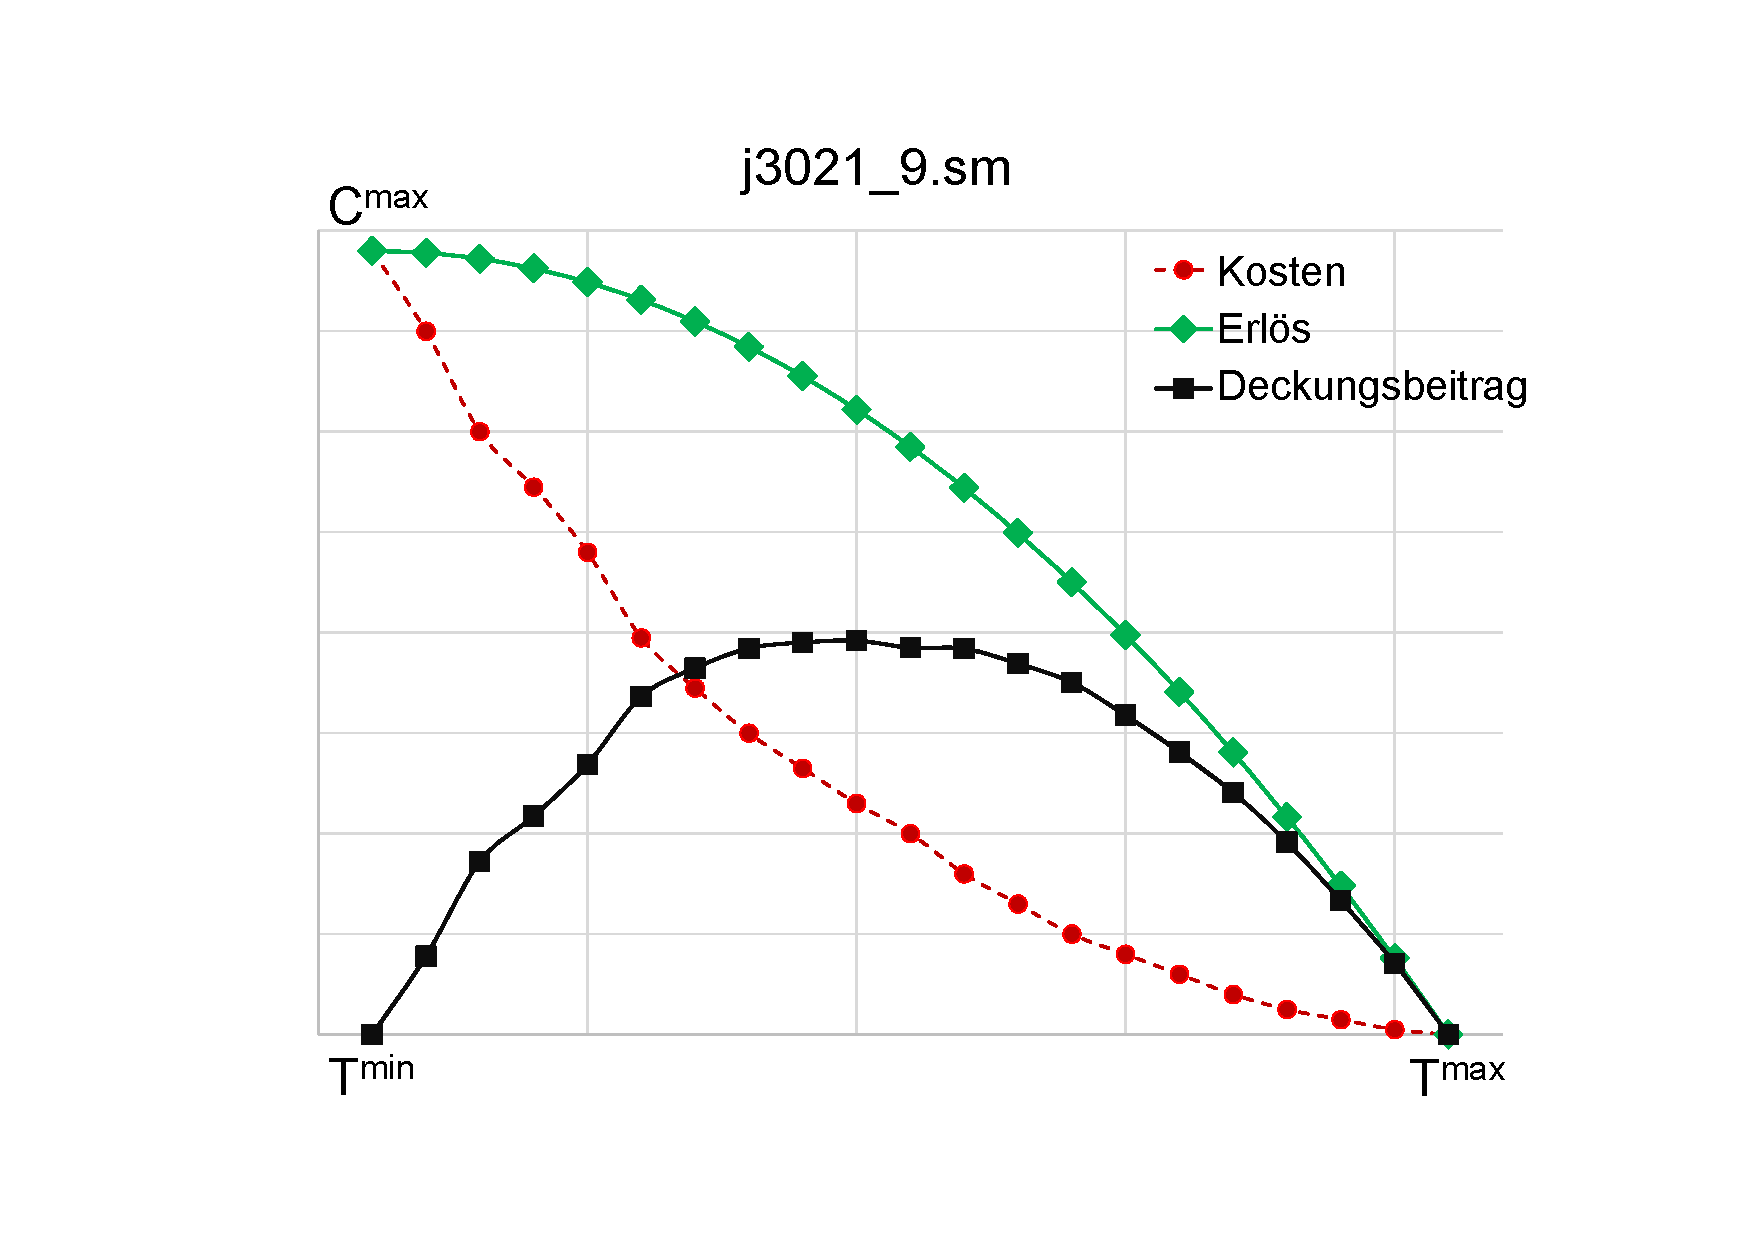
\includegraphics[scale=0.26]{images/DeadlineCosts.pdf}
\end{center}

\end{frame}


\begin{frame}
\frametitle{Parameter der Erlösfunktion}
\begin{itemize}
\item Problem: Bestimmung von $C^{\mbox{max}}$, $T^{\mbox{min}}$, $T^{\mbox{max}}$ erfordert Lösung eines RCPSP\\[5mm]
\item[$\rightarrow$]  Abschätzung mittels unterer bzw. oberer Schranken\\[2mm]
\begin{itemize}
\item $T^{\mbox{min}} \geq \mbox{max}\{EFT_{J},\mbox{max}_{r}\{\lceil\frac{\sum_{j}d_{j}k_{jr}}{K_{r}+\overline{z}_{r}}\rceil\}\}$\\[1mm]
\item $T^{\mbox{max}} \leq$ Dauer von SSGS-Ablaufplan mit $z_{rt}=0$\\[4mm]
\item $C^{\mbox{max}} \leq $ Kosten des $\mathcal{ESS}$
\end{itemize}
\end{itemize}
\end{frame}

\begin{frame}
\frametitle{Basis für Testinstanzen}
\begin{itemize}
\item Project Scheduling Problem Library (PSPLIB)
	\begin{itemize}
		\item RCPSP-Testinstanzen mit 30, 60, 90 und 120 AG
		\item Instanzgenerator PROGEN
		\item Beste bekannte Lösungen (Optimal für j30) für $T^{\mbox{max}}$\\[4mm]
	\end{itemize}

\item Erweiterung um $\kappa_r, \overline{z}_r$ und $u_t$\\[4mm]

\item Entferne Instanzen mit $T^{\mbox{min}} = T^{\mbox{max}}$
	\begin{itemize}
	\item $T^{\mbox{min}}$ kürzeste Projektdauer bei maximal möglicher ZK
	\item $T^{\mbox{max}}$ kürzeste Projektdauer bei keiner ZK
	\end{itemize}
\item Lösung von zwei RCPSPs je Testinstanz notwendig $\implies$ nur für $\lesssim 30$ AG praktikabel
\end{itemize}

\end{frame}

\begin{frame}
\frametitle{Berechnung optimaler Lösungen\\als Referenzwerte}
\begin{itemize}
\item Aktuell nur für 30 Arbeitsgänge\\[4mm]
\item GAMS-Implementierung von
	\begin{itemize}
	\item RCPSP-OC-Modell sowie
	\item RCPSP-Modell zur Berechnung von $T^{\mbox{min}}$\\[4mm]
	\end{itemize}
\item Für RCPSP-OC erweiterte j30-Testinstanzen in GDX-Format umgewandelt
\item Exakte Lösung per GUROBI parallel auf RRZN-Cluster
\item Problemspezifischer Branch\&Bound-Algorithmus
\end{itemize}
\end{frame}

\begin{frame}
\frametitle{Umsetzung der Genetischen Algorithmen}
\begin{itemize}
\item Implementierung in Delphi\\[4mm]
\item Großer Flaschenhals in $(\lambda)$-Repräsentation laut Profiling: Fitnessberechnung 
\begin{itemize}\item[$\rightarrow$] in Threads parallelisiert\\[4mm]\end{itemize}
\item Heuristik-Ausführung auf Cluster
\begin{itemize}
	\item Hoher Zeitbedarf für Gesamtevaluation:
		\begin{itemize}
		\item 12 Heuristiken
		\item 3*480 und 1*600 Projekte
		\item 1s, 2s, 10s, 15s Zeitlimit (für j30, j60, u.s.w.)
		\item[$\implies$] = $12 \cdot (480\cdot (1s + 2s + 10s) + 600\cdot15s ) = 50{,}8$ Stunden
		\end{itemize}
	\item Vergleichbarkeit
	\item Parallelisierte Berechnung gesamter Problembibliothek
\end{itemize}
\end{itemize}
\end{frame}

\section{Numerische Ergebnisse}
\begin{frame}
\frametitle{Gliederung}
\tableofcontents[current] %, hidesubsections]
\end{frame}


\begin{frame}[t]
\frametitle{Numerische Ergebnisse}
\begin{footnotesize}
\textbf{Parameter:} Zeitlimit$=\only<1>{1}\only<2>{2}\only<3>{10}\only<4>{15}s$, Populationsgröße$=80$, $P_{mutate}=5\%$\\
\only<1>{\textbf{Testinstanzen:} PSPLIB, j30 (30+2 Aktivitäten)\\199 optimal in $<$2 Stunden lösbare kapazitätsbeschränkte Projekte}
\only<2>{\textbf{Testinstanzen:} PSPLIB, j60 (60+2 Aktivitäten)\\480 Projekte}
\only<3>{\textbf{Testinstanzen:} PSPLIB, j90 (90+2 Aktivitäten)\\480 Projekte}
\only<4>{\textbf{Testinstanzen:} PSPLIB, j120 (120+2 Aktivitäten)\\600 Projekte}

\begin{center}

\begin{tabular}{ccccccccccccc}
\hline
representation & $(\lambda|z_{rt})$ & $(\lambda|z_r)$ & $(\lambda|\beta^{lsu})$ & $(\lambda|\beta^{Lsu})$ & $(\lambda|\beta^{lSu})$ & $(\lambda|\beta^{LSu})$ & $(\lambda|\beta^{lsU})$ & $(\lambda|\beta^{LsU})$ & $(\lambda|\beta^{lSU})$ & $(\lambda|\beta^{LSU})$ & $(\lambda|\tau)$ & $(\lambda)$\\[3pt]
\hline
$\varnothing$ deviation&1.41\%&3.01\%&2.80\%&2.91\%&3.35\%&3.75\%&4.16\%&4.19\%&4.92\%&5.27\%&2.45\%&1.20\%\\
\hline
max. deviation&8.83\%&45.00\%&45.00\%&45.00\%&45.00\%&45.00\%&45.00\%&45.00\%&45.00\%&45.00\%&20.23\%&14.29\%\\
\hline
varcoeff(dev)&1.45&1.77&1.94&1.88&1.61&1.50&1.61&1.61&1.33&1.27&1.30&1.69\\
\hline
\% optimal&46.73\%&28.64\%&29.65\%&30.15\%&28.64\%&28.14\%&24.62\%&25.13\%&20.60\%&21.11\%&41.21\%&52.76\%\\
\hline
\# best&116&70&74&72&65&60&60&62&44&46&94&128\\
\hline
$\varnothing$ rank&1.98&2.60&2.37&2.54&3.15&3.52&3.14&3.24&4.12&4.39&2.98&1.78\\\hline
\end{tabular}

\end{center}
\end{footnotesize}
\end{frame}

\begin{frame}
\frametitle{Konvergenzverhalten}
\includegraphics<1>[page=1, scale=0.69]{images/Convergence3011_7.pdf}
\end{frame}

\section{Ausblick}

\begin{frame}
\frametitle{Gliederung}
\tableofcontents[current] %, hidesubsections]
\end{frame}

\begin{frame}
\frametitle{Ausblick}
\begin{itemize}
\item Heuristische Methoden
	\begin{itemize}
	\item Integration weiterer Elemente führender RCPSP-Heuristiken
		\begin{itemize}
		\item Vorwärts-Rückwärts-Verbesserung
		\item Peak-Crossover
		\item Zweite Suchphase in Nachbarschaft
		\end{itemize}
	\item Stellschrauben im genetischen Algorithmus:\\$N^G$, $N^I$, $P_{mutate}$, genetische Operatoren\\[4mm]
	\end{itemize}
	
\item Exakte Methoden
	\begin{itemize}\item Problemspezifischer Branch\&Bound-Algorithmus\\[4mm]\end{itemize}
	
\item Problemgeneralisierung
	\begin{itemize}
	\item Zeitabhängige Ressourcenbelastungen $k_{jr\tau}$
	\item Mehr-Modus-Fall
	\item Flexible Projekte
	\end{itemize}
\end{itemize}
\end{frame}




